\documentclass[10pt,a4paper]{article}

\usepackage[a4paper,top=18mm,bottom=18mm,left=18mm,right=18mm]{geometry}
\usepackage[T1]{fontenc}
\usepackage{lmodern,microtype}
\usepackage{amsmath,amssymb,mathtools,bm}
\usepackage{xcolor,booktabs,tabularx,array,enumitem,multicol,graphicx}
\usepackage{tikz}
\usetikzlibrary{arrows.meta,positioning,calc}
\usepackage[most]{tcolorbox}
\usepackage{fancyhdr,hyperref}
\definecolor{ink}{HTML}{24354B}
\definecolor{accent}{HTML}{135E77}
\definecolor{pale}{HTML}{F1F7F8}
\hypersetup{colorlinks=true,linkcolor=accent,urlcolor=accent,pdfauthor={PHYS4055 revision notes}}
\setlength{\parindent}{0pt}
\setlength{\parskip}{4pt}
\setlength{\emergencystretch}{3em}
\setlist{leftmargin=*,topsep=2pt,itemsep=1pt}
\AtBeginDocument{\color{ink}}
\pagestyle{fancy}
\fancyhf{}
\fancyhead[L]{\footnotesize PHYS4055 \textbar\ Exam Revision}
\fancyhead[R]{\footnotesize 2026 \textbar\ Open-book notes}
\fancyfoot[C]{\footnotesize\thepage}
\renewcommand{\headrulewidth}{0.3pt}
\newcommand{\ket}[1]{\left\lvert #1\right\rangle}
\newcommand{\bra}[1]{\left\langle #1\right\rvert}
\newcommand{\braket}[2]{\left\langle #1\middle\vert #2\right\rangle}
\newcommand{\mel}[3]{\left\langle #1\middle\vert #2\middle\vert #3\right\rangle}
\newcommand{\diff}{\mathrm{d}}
\newcommand{\ii}{\mathrm{i}}
\newcommand{\e}{\mathrm{e}}
\newtcolorbox{methodbox}{colback=pale,colframe=accent!50!white,boxrule=0.4pt,arc=1mm,before skip=5pt,after skip=5pt}
\newtcolorbox{cautionbox}{colback=white,colframe=black!20,boxrule=0.4pt,arc=1mm,before skip=5pt,after skip=5pt}

\usepackage{titlesec}
\usepackage{listings}
\geometry{top=17mm,bottom=17mm,left=17mm,right=17mm,headsep=6mm,footskip=8mm}
\hypersetup{pdftitle={PHYS4055 - All Four Assignments, Complete Worked Solutions (2026)}}
\setlength{\parskip}{3pt plus 0.4pt minus 0.2pt}
\setlength{\emergencystretch}{3em}
\renewcommand{\arraystretch}{1.14}
\titleformat{\section}{\large\bfseries\color{accent}}{\thesection}{0.6em}{}
\titlespacing*{\section}{0pt}{14pt plus 3pt}{7pt}
\newcommand{\assignq}[4]{\section[Assignment #1 Q#2: #3]{Question #2: #3}
{\footnotesize\color{gray}Source: PHYS4055 2026 Assignment #1,
Question #2, source question-sheet page(s) #4.}\par\vspace{4pt}}
\newcommand{\assignmentpart}[2]{\clearpage
\phantomsection\addcontentsline{toc}{part}{Assignment #1: #2}
\noindent{\color{accent}\LARGE\bfseries Assignment #1}\par
\vspace{2pt}{\color{accent}\large #2}\par\vspace{4pt}\hrule\vspace{9pt}}
\newcommand{\methodnote}[1]{\begin{methodbox}
\footnotesize\textbf{Exam method / verification.} #1
\end{methodbox}}
\begin{document}
\begin{center}
\vspace*{7mm}
{\color{accent}\Huge\bfseries PHYS4055}\\[3mm]
{\LARGE Atomic Physics and Quantum Optics}\\[7mm]
{\Large\bfseries Complete Worked Assignment Solutions}\\[3mm]
{\Large Assignments 1--4}\\[5mm]
{\normalsize All 12 primary questions, with every subpart}\\[3mm]
{\normalsize Source-grounded 2026 revision edition}
\end{center}
\vspace{8mm}
\begin{methodbox}
\textbf{Aim.} A step-by-step companion to the
15-page course overview and the 20-example revision book.
Every assignment question is unpacked into its physics model,
working and final result. Numerical calculations for
\(^{209}\mathrm{Bi}\) and neutral Na are accompanied by a
reproducible, separately versioned Python script.
\end{methodbox}

\begin{center}
\begin{tabularx}{\linewidth}{@{}p{31mm}p{15mm}X@{}}
\toprule
\textbf{Assignment}&\textbf{Questions}&\textbf{Main subjects}\\\midrule
1: Quantum optics&2&
Two-mode squeezed vacuum, thermal marginal,
photon pair correlations, beam splitters,
coherent-state outputs and photon counting\\
2: Applications of optics&3&
Bell states, partial traces, dense coding,
Bell-state detection and BB84 QKD\\
3: Atomic physics&4&
Finite nuclear radius, \(d^2\) terms and NIST
spectra, Stark polarisability, Land\'e factors\\
4: Atomic applications&3&
Hartree--Fock direct/exchange derivation,
Zeeman slowing, Na numerical radiative lifetimes\\
\bottomrule
\end{tabularx}
\end{center}
\bigskip
\begin{cautionbox}
\textbf{Authority and limitations.}
The question sheets are included in
\texttt{source\_material/assignments/questions}.
Official worked solutions have been released
for Assignments \textbf{1 and 2}; their methods
are cross-checked here. Official solutions for
Assignments \textbf{3 and 4} were not in the uploaded
material: those answers are independently derived.
All external atomic constants, data and caveats
are documented in \texttt{SOURCE\_MAP.md}.
\end{cautionbox}
\vfill
\noindent{\footnotesize First version: 14 November 2026.
For numerical work run
\texttt{python scripts/assignment\_numerical\_solutions.py}
from the repository root.}
\clearpage
\tableofcontents

\assignmentpart{1}{Introduction to quantum optics}

\assignq{1}{1}{Two-mode squeezed vacuum: thermal reductions and heralding}{1}
The input state is
\[
\ket{\Psi}_{si}=\sqrt{1-\lambda^2}\sum_{n=0}^\infty
\lambda^n\ket n_s\ket n_i,\qquad \lambda=\tanh r.
\]
\subsection*{(a) Partial trace and mean occupation}
Expand the joint density operator:
\[
\rho_{si}=(1-\lambda^2)\sum_{m,n}
\lambda^{m+n}\ket m_s\bra n_s\otimes\ket m_i\bra n_i.
\]
The identity \(\operatorname{Tr}_i(\ket m\bra n)=\delta_{mn}\)
makes all off-diagonal signal terms disappear:
\[
\boxed{\rho_s=(1-\lambda^2)\sum_{n=0}^\infty
\lambda^{2n}\ket n\bra n}.
\]
The same holds for the idler.
Put \(q=\lambda^2\) so \(p_n=(1-q)q^n\).
From \(\sum q^n=(1-q)^{-1}\), differentiation gives
\[
\bar n=(1-q)\sum_{n=0}^\infty nq^n
=\boxed{\frac{\lambda^2}{1-\lambda^2}=\sinh^2r}.
\]
Since \(q=\bar n/(1+\bar n)\),
\(p_n=\bar n^n/(1+\bar n)^{n+1}\), the single-mode
thermal photon-number distribution.
The \emph{joint} state is pure while each subsystem
is a mixed thermal state.

\subsection*{(b) Cross-correlation}
Signal and idler have identical photon numbers in
each Schmidt term, so \(\langle n_sn_i\rangle=\langle n^2\rangle\).
Use
\(\sum n^2q^n=q(1+q)/(1-q)^3\):
\[
\langle n_sn_i\rangle
=\frac{q(1+q)}{(1-q)^2}
=\bar n+2\bar n^2.
\]
Therefore
\[
\boxed{g^{(2)}_{si}(0)
=\frac{\langle n_sn_i\rangle}{\bar n^2}
=2+\frac1{\bar n}}.
\]
As \(r\to0^+\), pairs become rare but very highly
correlated, so the normalised function diverges.
At exactly \(\bar n=0\), it is undefined (zero denominator).

\subsection*{(c) Herald a single photon}
At low gain,
\(\ket{\Psi}\approx\ket{0,0}+\lambda\ket{1,1}
+O(\lambda^2)\).
An idler outcome \(\bra1_i\) leaves an unnormalised
signal amplitude proportional to \(\lambda\ket1_s\).
After normalisation,
\[
\boxed{\rho_{s\mid n_i=1}=\ket1\bra1}.
\]
A threshold detector is a good herald only when
multi-pair events are negligible; ideal number
resolution would isolate the one-pair component exactly.
\methodnote{Differentiate the geometric series;
do not confuse a local thermal state with an absence
of correlations in the joint entangled state.}


\assignq{1}{2}{Beam splitter on Fock and coherent inputs}{1}
The input/output relation is the real rotation
\[
\begin{pmatrix}c\\d\end{pmatrix}
=\begin{pmatrix}\tau&-\varrho\\\varrho&\tau\end{pmatrix}
\begin{pmatrix}a\\b\end{pmatrix}.
\]
Unitarity means \(\tau^2+\varrho^2=1\).
The coefficients appearing in the \emph{matrix}
are field-amplitude coefficients: the corresponding
intensity fractions are \(\tau^2,\varrho^2\).

\subsection*{(a) The binomial transformation}
The inverse mode relation gives
\(a^\dagger=\tau c^\dagger+\varrho d^\dagger\).
Write the number state with creation operators:
\[
\ket{n,0}_{ab}=\frac{(a^\dagger)^n}{\sqrt{n!}}\ket0.
\]
Expand the commuting creation operators:
\[
\frac1{\sqrt{n!}}\sum_{k=0}^n\binom nk
\tau^k\varrho^{n-k}
(c^\dagger)^k(d^\dagger)^{n-k}\ket0.
\]
Because the normalised number states satisfy
\((c^\dagger)^k(d^\dagger)^{n-k}\ket0
=\sqrt{k!(n-k)!}\ket{k,n-k}\), this becomes
\[
\boxed{\ket{n,0}_{ab}\longrightarrow
\sum_{k=0}^n
\sqrt{\frac{n!}{k!(n-k)!}}\,
\tau^k\varrho^{n-k}\ket{k,n-k}_{cd}}.
\]
Normalisation follows from
\(\sum_k\binom nk\tau^{2k}\varrho^{2(n-k)}
=(\tau^2+\varrho^2)^n=1\).

\subsection*{(b) Coherent input plus vacuum}
For \(c=(a+b)/\sqrt2,\ d=(a-b)/\sqrt2\),
write the input as
\[
\ket{\alpha,0}=e^{-|\alpha|^2/2}
\exp(\alpha a^\dagger)\ket0.
\]
The inverse relation is
\(a^\dagger=(c^\dagger+d^\dagger)/\sqrt2\).
The two output creation operators commute, so
the exponential factors:
\[
\begin{aligned}
\ket{\Psi_{\rm out}}
&=e^{-|\alpha|^2/2}
e^{(\alpha/\sqrt2)c^\dagger}
e^{(\alpha/\sqrt2)d^\dagger}\ket0\\
&=\boxed{\ket{\alpha/\sqrt2}_c\otimes
\ket{\alpha/\sqrt2}_d}.
\end{aligned}
\]
Phase conventions can change the sign of one
amplitude without changing output count statistics.

\subsection*{(c) Photodetection}
The \(c\)-mode coherent amplitude is
\(\beta=\alpha/\sqrt2\).
Thus
\[
\boxed{P_c(n)=
e^{-|\alpha|^2/2}\frac{(|\alpha|^2/2)^n}{n!}},
\qquad
\boxed{\langle n_c\rangle=\operatorname{Var}(n_c)
=\frac{|\alpha|^2}{2}}.
\]
The ideal detector observes \emph{Poissonian} counts.
\methodnote{Normalised Fock coefficients need the
square roots of factorials; keep amplitude and intensity
transmission coefficients distinct.}


\assignmentpart{2}{Quantum optics applications}

\assignq{2}{1}{Bell states: orthonormality, reduced state and correlations}{1}
We encode \(\ket0=\ket H\), \(\ket1=\ket V\) and define
\[
\ket{\Phi^\pm}=\frac{\ket{00}\pm\ket{11}}{\sqrt2},
\qquad
\ket{\Psi^\pm}=\frac{\ket{01}\pm\ket{10}}{\sqrt2}.
\]
\subsection*{(a) Check every Bell-state overlap}
Write \(s,t\in\{+1,-1\}\) and
\(\ket{\Phi_s}=(\ket{00}+s\ket{11})/\sqrt2\).
Orthonormality of the computational basis gives
\[
\braket{\Phi_s}{\Phi_t}
=\frac12(1+st)
=\begin{cases}1&s=t\\0&s\ne t.\end{cases}
\]
Exactly the same reasoning gives
\(\braket{\Psi_s}{\Psi_t}=\delta_{st}\).
The two families use disjoint computational-basis
states, so \(\braket{\Phi_s}{\Psi_t}=0\).
Thus \(\boxed{\braket{B_i}{B_j}=\delta_{ij}}\)
for all four Bell states.

\subsection*{(b) Reduced density matrix of photon \(A\)}
For \(\ket{\Phi^+}\),
\[
\begin{aligned}
\rho_{AB}=\tfrac12(&\ket{00}\bra{00}
+\ket{00}\bra{11}\\
&+\ket{11}\bra{00}+\ket{11}\bra{11}).
\end{aligned}
\]
Use
\(\operatorname{Tr}_B(\ket{i,j}\bra{k,l})
=\delta_{jl}\ket i\bra k\).
The cross terms vanish and the diagonal terms survive:
\[
\boxed{\rho_A=\frac{\ket0\bra0+\ket1\bra1}{2}
=\frac12I}.
\]
Therefore \(P(H)=P(V)=1/2\) for measurements
on \(A\) alone. Its purity
\(\operatorname{Tr}\rho_A^2=1/2<1\) shows a
mixed local state, though \(\rho_{AB}\) is pure.

\subsection*{(c) Repeat in the diagonal-polarisation basis}
Define
\(\ket D=(\ket H+\ket V)/\sqrt2\),
\(\ket A=(\ket H-\ket V)/\sqrt2\).
Hence
\(\ket H=(\ket D+\ket A)/\sqrt2\),
\(\ket V=(\ket D-\ket A)/\sqrt2\).
Substitution and cancellation of the two cross terms yields
\[
\ket{HH}+\ket{VV}=\ket{DD}+\ket{AA},
\quad
\boxed{\ket{\Phi^+}
=\frac{\ket{DD}+\ket{AA}}{\sqrt2}}.
\]
Both observers using \(H/V\) obtain
\((H,H)\) or \((V,V)\), each with probability \(1/2\).
Both using \(D/A\) obtain \((D,D)\) or \((A,A)\),
again each with probability \(1/2\).
The local outcomes are random but their
\emph{joint} outcomes are perfectly correlated.
\methodnote{Distinguish single-photon randomness
from two-photon correlation. The partial trace
must eliminate off-diagonal terms with unequal
\(B\)-indices.}


\assignq{2}{2}{Superdense coding and a passive linear-optical Bell measurement}{2--3}
Start with \(\ket{\Phi^+}_{AB}\) and act on
\emph{Alice's} qubit only. The problem defines
\(X\ket0=\ket1,\ X\ket1=\ket0\),
\(Z\ket0=\ket0,\ Z\ket1=-\ket1\).

\subsection*{(a) Calculate the four encoded Bell states}
Direct application to each computational term gives
\[
\begin{array}{c|c|c}
\text{message}&\text{gate on }A&\text{output state}\\\hline
00&I&(\ket{00}+\ket{11})/\sqrt2=\ket{\Phi^+}\\
01&X&(\ket{10}+\ket{01})/\sqrt2=\ket{\Psi^+}\\
10&Z&(\ket{00}-\ket{11})/\sqrt2=\ket{\Phi^-}\\
11&XZ&(\ket{10}-\ket{01})/\sqrt2=-\ket{\Psi^-}
\end{array}
\]
The last global minus phase is unobservable, so
the four encodings specify four orthogonal Bell states.

\subsection*{(b) Why two bits can be sent}
Before communication, Alice and Bob share
one entangled Bell pair. Alice chooses one
of four unitaries (\(2^2\) alternatives), sends
her \emph{one} photon, and Bob performs an
ideal joint Bell-basis measurement.
Four orthogonal outputs encode two classical bits.
The shared entanglement and the transmitted
physical qubit together provide the resource;
this is not two bits from an arbitrary isolated
one-photon qubit.

\subsection*{(c) Expand the specified beam-splitter measurement}
For each polarisation label \(\lambda=H,V\),
\[
a_\lambda^\dagger\longrightarrow
\frac{c_\lambda^\dagger+d_\lambda^\dagger}{\sqrt2},
\qquad
b_\lambda^\dagger\longrightarrow
\frac{c_\lambda^\dagger-d_\lambda^\dagger}{\sqrt2}.
\]
For two equal polarisations,
\(a_\lambda^\dagger b_\lambda^\dagger
\to[(c_\lambda^\dagger)^2-
(d_\lambda^\dagger)^2]/2\). Therefore
\[
\boxed{\ket{\Phi^\pm}\longrightarrow
\frac{(c_H^\dagger)^2-(d_H^\dagger)^2
\pm(c_V^\dagger)^2\mp(d_V^\dagger)^2}
{2\sqrt2}\ket{\mathrm{vac}}}.
\]
For the \(\Psi\) states the mixed-polarisation
amplitudes interfere:
\[
\boxed{\ket{\Psi^+}\longrightarrow
\frac{c_H^\dagger c_V^\dagger
-d_H^\dagger d_V^\dagger}{\sqrt2}
\ket{\mathrm{vac}}},\qquad
\boxed{\ket{\Psi^-}\longrightarrow
\frac{c_V^\dagger d_H^\dagger
-c_H^\dagger d_V^\dagger}{\sqrt2}
\ket{\mathrm{vac}}}.
\]
A polarising beam splitter and number-resolving detectors
at each output distinguish these patterns:
\[
\begin{array}{c|l|c}
\text{Bell input}&\text{Detection signature}&
\text{Identification}\\\hline
\Phi^+&2\text{ photons same port, same pol.}&
\text{ambiguous}\\
\Phi^-&2\text{ photons same port, same pol.}&
\text{ambiguous}\\
\Psi^+&2\text{ orthogonal pol., same port}&
\text{unique}\\
\Psi^-&1\text{ photon each port, orthogonal pol.}&
\text{unique}
\end{array}
\]
The relative signs between \(\Phi^\pm\) components
do not change these photon-count patterns.

\subsection*{(d) Decoding efficiency}
With four equiprobable messages, only
\(\Psi^+,\Psi^-\) are unambiguous:
\[
\boxed{P_{\mathrm{unambiguous}}=\frac24=\frac12}.
\]
Thus the standard passive linear-optical analyser
alone cannot implement a \emph{deterministic}
four-outcome Bell measurement. Extra
ancillary resources or different physical
interactions may improve the measurement.
\methodnote{Bosonic operators for distinct modes commute.
Add coherent creation-operator amplitudes before converting
into Fock-state probabilities.}


\assignq{2}{3}{BB84: preparation, sifting, intercept--resend and key distillation}{3--4}
\subsection*{(a) Encode bit and basis}
The agreed logical encoding is
\[
\begin{array}{c|cc}
\text{bit}&Z\ \text{basis}&X\ \text{basis}\\\hline
0&\ket H&\ket D=(\ket H+\ket V)/\sqrt2\\
1&\ket V&\ket A=(\ket H-\ket V)/\sqrt2
\end{array}
\]
These two bases are mutually unbiased:
for example \(|\braket{H}{D}|^2=1/2\).

\subsection*{(b) Sift the key and account for loss}
Alice and Bob choose each basis with probability \(1/2\).
The probability of matching choices is
\[
P(\text{match})=P(ZZ)+P(XX)=\tfrac14+\tfrac14
=\boxed{\tfrac12}.
\]
A single photon is detected with probability
\(\eta_{\mathrm{ch}}\eta_d\), assuming no
dark counts or other imperfections:
\[
\boxed{\mathbb{E}[N_{\mathrm{det}}]
=N\eta_{\mathrm{ch}}\eta_d},\qquad
\boxed{\mathbb{E}[N_{\mathrm{sift}}]
=\tfrac12N\eta_{\mathrm{ch}}\eta_d}.
\]
The sifted-key expectation refers to detected
photons for which their announced bases agree.

\subsection*{(c) Derive the error from intercept--resend}
Compute the quantum bit error rate \emph{conditioned}
on Alice and Bob having used the same basis.
Eve chooses that basis with probability \(1/2\);
she then learns and resends the bit without error.
With probability \(1/2\), Eve chooses the
conjugate basis. Her outcome is random relative
to Alice; when Bob measures in Alice's basis
he obtains the wrong bit with probability \(1/2\).
Thus
\[
\boxed{Q=\tfrac12(0)+\tfrac12(\tfrac12)
=\frac14=25\%.}
\]
This is an ideal single-photon intercept--resend
attack, not a universal error rate for every attack.

\subsection*{(d.i) Probability of seeing an error}
For \(m=20\) independently sampled sifted bits,
\[
\boxed{P(\text{at least one error})
=1-(1-Q)^m=1-\left(\frac34\right)^{20}
=0.99683\ \text{(about }99.68\%\text{)}.}
\]

\subsection*{(d.ii) Why discard public test bits?}
The comparison exposes each tested bit on the
authenticated public channel. Eve can therefore
know their values, so the publicly revealed bits
cannot be part of the secret final key.

\subsection*{(d.iii) The two final processing steps}
\textbf{Error correction} reconciles any
differences between Alice's and Bob's sifted
strings, using public parity/syndrome
information as necessary. This discussion
also leaks some information.
\textbf{Privacy amplification} compresses the
reconciled string with an appropriate hash
function to reduce a potential eavesdropper's
remaining information to a negligible level.
\methodnote{Do not apply the basis-sifting factor
twice. For an intercept--resend QBER always
condition on a basis match between Alice and Bob.}


\assignmentpart{3}{Atomic physics}
\assignq{3}{1}{Finite nuclear size of hydrogen-like \(^{209}\mathrm{Bi}\)}{1}
Work in atomic units. A point-nucleus Coulomb potential is
\(V_0=-Z/r\), while the specified uniform sphere has
\[
V_R(r)=
\begin{cases}
-\frac Z{2R}(3-r^2/R^2)&r<R,\\
-Z/r&r\ge R.
\end{cases}
\]
Thus the perturbation is
\[
\Delta V(r)=Z\left(\frac1r-\frac3{2R}
+\frac{r^2}{2R^3}\right)\quad(r<R),
\]
and zero for \(r\ge R\).

\subsection*{(a) Derive the leading \(s\)-state correction}
First-order perturbation theory yields
\[
\Delta E_{ns}^{(1)}
=\mel{ns}{\Delta V}{ns}
\simeq4\pi|\psi_{ns}(0)|^2\int_0^R
r^2\Delta V(r)\diff r .
\]
For hydrogenic \(s\)-states,
\(|\psi_{ns}(0)|^2=Z^3/(\pi n^3)\).
Perform the radial integral explicitly:
\[
\begin{aligned}
\int_0^R r^2\Delta V(r)\diff r
&=Z\left[\frac{R^2}{2}
-\frac{3R^2}{6}+\frac{R^2}{10}\right]\\
&=\frac{ZR^2}{10}.
\end{aligned}
\]
Hence
\[
\boxed{\Delta E_{ns}^{\rm fns}
=\frac{2Z^4R^2}{5n^3}
=\frac{2Z^2}{5n^3}(ZR)^2\quad(\text{Hartree})}.
\]
It is positive: spreading out the nuclear charge
weakens the strongly attractive potential near the origin.

\subsection*{(b) Numerical integrals for \(^{209}\mathrm{Bi}^{82+}\)}
The nuclear charge is \(Z=83\). With
\(R_{\rm rms}=5.5211\,\mathrm{fm}\), take
\[
R=\sqrt{\frac53}R_{\rm rms}=7.1277\,\mathrm{fm}
=1.34694\times10^{-4}a_0.
\]
Use normalised hydrogenic \(R_{nl}(r)\) and integrate
\[
\boxed{\Delta E_{nl}=\int_0^R
|R_{nl}(r)|^2r^2\Delta V(r)\diff r}.
\]
The accompanying Python solver performs this
quadrature rather than assuming that all \(l\) give
the same \(s\)-state correction:
\[
\begin{array}{c|r|r}
\text{State}&\Delta E_{\rm fns}\ (\mathrm{Ha})&
\Delta E_{\rm fns}\ (\mathrm{eV})\\\hline
1s&0.3412153&9.28494\\
2p&9.54585\times10^{-8}&2.59756\times10^{-6}\\
3d&8.63359\times10^{-15}&2.34932\times10^{-13}
\end{array}
\]
The leading-order \(1s\) formula gives
\(0.3444055\,\mathrm{Ha}\), approximately
\(0.94\%\) higher than numerical first-order
Schr\"odinger perturbation theory. The higher
angular momenta are strongly suppressed near
the nuclear region because \(R_{nl}\sim r^l\).

\subsection*{(c) Relativistic comparison}
The exact \emph{point-nucleus} Dirac Coulomb
energy (excluding rest mass) is
\[
E_{n\kappa}^{D}=\frac1{\alpha_{\rm fs}^2}
\left[
\left(1+\frac{(Z\alpha_{\rm fs})^2}
{(n-|\kappa|+\sqrt{\kappa^2-(Z\alpha_{\rm fs})^2})^2}
\right)^{-1/2}-1\right]\ {\rm Ha}.
\]
Compare with \(E_n^{NR}=-Z^2/(2n^2)\):
\[
\begin{array}{c|r|r}
\text{Fine-structure level}&
E^{D}-E^{NR}\ (\mathrm{Ha})&
\Delta E_{\rm fns}^{NR}\ (\mathrm{Ha})\\\hline
1s_{1/2}&-391.87&0.3412\\
2p_{1/2}&-123.80&9.55\times10^{-8}\\
3d_{3/2}&-12.31&8.63\times10^{-15}
\end{array}
\]
The relativistic shifts are far larger than
these \emph{nonrelativistic} finite-nucleus
perturbation results. This is not a precision
relativistic heavy-ion calculation:
\(Z\alpha_{\rm fs}\simeq0.606\), so the real
Dirac radial functions have significantly
different nuclear-region amplitudes.
\methodnote{Numerical source:
\texttt{scripts/assignment\_numerical\_solutions.py}.
For \(R_{nl}\) use \(r^2\diff r\); for
\(u=rR_{nl}\) use \(\diff r\).}

\assignq{3}{2}{Equivalent \(d^2\) electrons and NIST Ti I spectra}{1}
\subsection*{(a) Enumerate the terms}
There are \(5(2)=10\) available \(d\)-electron spin-orbitals,
and \(\binom{10}{2}=45\) antisymmetrised pairs.
Coupling \(l_1=l_2=2\) permits \(L=0,\ldots,4\);
two spins allow \(S=0\) (antisymmetric) or \(S=1\)
(symmetric). Orbital exchange symmetry is
\((-1)^{2l-L}=(-1)^L\). Consequently even \(L\)
requires singlet spin and odd \(L\) requires
triplet spin. Attach \(J=|L-S|,\ldots,L+S\):
\[
\boxed{
{}^1S_0,\ {}^1D_2,\ {}^1G_4,\
{}^3P_{0,1,2},\ {}^3F_{2,3,4}.}
\]
The check
\(1+5+9+(1+3+5)+(5+7+9)=45\)
recovers all permitted microstates.

\subsection*{(b) Hund's ordering}
Maximise \(S\), then \(L\). For a less-than-half
filled shell, lowest \(J\) lies lowest within
each term:
\[
\boxed{\text{ground }{}^3F_2,\quad
{}^3F_2<{}^3F_3<{}^3F_4,\quad
{}^3P_0<{}^3P_1<{}^3P_2.}
\]
These rules do not predict an exact ranking
between \emph{all different excited terms}.

\subsection*{(c) NIST Ti I data}
Neutral Ti has configuration
\([\mathrm{Ar}]3d^24s^2\).
The NIST Ti I levels for this configuration are:
\[
\begin{array}{c|r@{\quad}c|r}
\text{Level}&\mathrm{cm}^{-1}&\text{Level}&\mathrm{cm}^{-1}\\\hline
{}^3F_2&0.000&{}^3F_3&170.134\\
{}^3F_4&386.875&{}^1D_2&7255.354\\
{}^3P_0&8436.617&{}^3P_1&8492.421\\
{}^3P_2&8602.342&{}^1G_4&12118.394
\end{array}
\]
The ground term and within-multiplet \(J\) orders
agree with Hund's predictions. The observed
\({}^1D_2\) singlet, however, lies \emph{below}
the \({}^3P\) triplet, so the simplistic global
triplet/singlet ranking fails. The allowed
\({}^1S_0\) term is not identified in this
short NIST handbook table, and its energy
cannot be asserted from these data.

\subsection*{(d) Convert a measured excitation energy}
Taking the \({}^1D_2\) excitation:
\[
\boxed{\Delta E=7255.354\,\mathrm{cm}^{-1}
=\frac{7255.354}{219474.63137}\,E_h
=0.0330578\,E_h}.
\]
The zero of energy is the atomic ground state,
not the ionisation limit.
\methodnote{NIST neutral Ti I levels:
\texttt{physics.nist.gov/PhysRefData/Handbook/Tables/
titaniumtable5.htm}. A microstate count is the
fastest way to detect missing or Pauli-forbidden terms.}

\assignq{3}{3}{Hydrogenic static polarisability from perturbation theory}{2}
\subsection*{(a) Approximate the \(1s\) polarizability}
For a uniform electric field in the \(z\) direction,
\(H'=-\mathbf d\cdot\boldsymbol{\mathcal E}
=e z\mathcal E\). The \(1s\) state has even
parity, so \(\langle1s|z|1s\rangle=0\):
its first-order Stark shift vanishes.
For a nondegenerate level, second-order
perturbation theory gives
\[
\Delta E^{(2)}=\mathcal E^2
\sum_{m\ne1}\frac{|\langle m|ez|1\rangle|^2}{E_1-E_m}
=-\tfrac12\alpha\mathcal E^2.
\]
In atomic units, therefore,
\[
\alpha=2\sum_{m\ne1}
\frac{|\langle m|z|1s\rangle|^2}{E_m-E_1}.
\]
Approximate every denominator by
\(E_2-E_1=3Z^2/8\) Hartree.
Closure, \(\sum_m\ket m\bra m=I\), gives
\[
\sum_{m\ne1}|\langle m|z|1s\rangle|^2
=\langle1s|z^2|1s\rangle
-|\langle1s|z|1s\rangle|^2
=\langle z^2\rangle.
\]
Spherical symmetry implies
\(\langle z^2\rangle=\langle r^2\rangle/3\).
For hydrogenic \(1s\),
\(\langle r^2\rangle=3/Z^2\), hence
\[
\boxed{\alpha_{\rm approx}=
\frac{2(1/Z^2)}{3Z^2/8}
=\frac{16}{3Z^4}\ a_0^3.}
\]

\subsection*{(b) Hydrogen: numerical comparison}
For \(Z=1\), \(\alpha_{\rm approx}=16/3=5.3333\ a_0^3\).
With \(a_0=5.2917721\times10^{-9}\,\mathrm{cm}\),
\[
\boxed{\alpha_{\rm approx}(H)
=5.3333\,a_0^3
=7.903\times10^{-25}\,\mathrm{cm}^3}.
\]
This is the standard \emph{polarizability-volume}
convention; the SI dipole polarizability is
\(4\pi\epsilon_0\) times this volume.
The exact hydrogen value is \(9a_0^3/2=4.5a_0^3\).
The approximate denominator overestimates it by
\[
\boxed{\frac{5.3333-4.5}{4.5}\times100\%
=18.52\%.}
\]

\subsection*{(c) Hydrogen-like rubidium}
For a nucleus of \(Z=37\) with \emph{one}
hydrogenic \(1s\) electron:
\[
\boxed{\alpha(\mathrm{Rb}^{36+})\approx
\frac{16}{3(37)^4}\,a_0^3
=2.846\times10^{-6}\,a_0^3
=4.217\times10^{-31}\,\mathrm{cm}^3}.
\]
Neutral Rb has outer \(5s\) valence electrons
which are far more weakly bound and more
spatially extended; its ground-state
polarisability (\(\sim319\,a_0^3\) as supplied)
is about \(1.12\times10^8\) times larger.
\methodnote{Parity makes the first-order
shift vanish. Closure converts a difficult
sum to a ground-state expectation value;
the approximate energy denominator is why
the result is not exact.}

\assignq{3}{4}{Land\'e factors: electronic and nuclear coupling}{2}
\subsection*{(a) Derive \(g_J\)}
Write \(\mathbf J=\mathbf L+\mathbf S\),
\(\boldsymbol\mu=-\mu_B(g_L\mathbf L+g_S\mathbf S)\)
in dimensionless angular-momentum units,
with \(g_L=1,\ g_S=2\).
Only the projection of \(\boldsymbol\mu\)
on \(\mathbf J\) contributes to the
weak-field diagonal energy in a fixed \(J\) manifold:
\[
g_J=\frac{\langle(g_L\mathbf L+g_S\mathbf S)
\cdot\mathbf J\rangle}{J(J+1)}.
\]
Using
\[
2\mathbf J\cdot\mathbf L
=\mathbf J^2+\mathbf L^2-\mathbf S^2,\quad
2\mathbf J\cdot\mathbf S
=\mathbf J^2+\mathbf S^2-\mathbf L^2,
\]
we find
\[
\boxed{g_J=1+
\frac{J(J+1)+S(S+1)-L(L+1)}{2J(J+1)}}
\quad (J>0).
\]

\subsection*{(b) Derive \(g_F\) neglecting nuclear magnetism}
Now \(\mathbf F=\mathbf I+\mathbf J\).
The electronic moment lies along \(\mathbf J\)
on average, while \(\mathbf J\) projects onto
\(\mathbf F\) with factor
\[
\frac{\langle\mathbf J\cdot\mathbf F\rangle}{F(F+1)}
=\frac{F(F+1)+J(J+1)-I(I+1)}{2F(F+1)}.
\]
Thus
\[
\boxed{g_F=g_J
\frac{F(F+1)+J(J+1)-I(I+1)}{2F(F+1)}},
\qquad F>0.
\]
This is the electronic contribution only;
the nuclear \(g_I\mu_N\) term was excluded
by the question's stated approximation.

\subsection*{(c) \({}^2P_{1/2}\) in a weak field}
Here \(L=1,\ S=1/2,\ J=1/2\) and
\[
g_J=1+\frac{3/4+3/4-2}{2(3/4)}
=\boxed{\frac23}.
\]
For \(I>0\), the coupled manifolds are
\(F_+=I+\tfrac12\) and \(F_-=I-\tfrac12\)
(the latter is \(F=0\) for \(I=1/2\)).
Substituting into the preceding expression
gives, for nonzero \(F\),
\[
\boxed{g_{I+1/2}=+\frac{2}{3(2I+1)},\qquad
g_{I-1/2}=-\frac{2}{3(2I+1)}}.
\]
The weak-field energies are
\[
\boxed{\Delta E_{Fm_F}=\mu_B g_Fm_FB},
\quad m_F=-F,\ldots,F.
\]
The upper/lower hyperfine multiplets
fan out into \(2F+1\) equally spaced
Zeeman levels with \emph{opposite} slopes.
For the common \(I=5/2\) example,
\(F=3,2\) with \(g_F=+1/9,-1/9\).
When \(F=0\), there is only \(m_F=0\)
and no first-order electronic Zeeman
splitting, so the formula defining \(g_{F=0}\)
should not be used.
\methodnote{Project angular momenta
sequentially \(L,S\to J\), then \(I,J\to F\).
In strong fields this coupled-\(F\) result
no longer applies without state mixing.}


\assignmentpart{4}{Applications of atomic physics}
\assignq{4}{1}{Hartree--Fock: direct and exchange Coulomb matrix elements}{1}
The task refers specifically to Johnson's closed-shell
results, Eqs.~(3.64) and (3.66). Here we derive both
from the multipole expansion, including the sum
over the \emph{occupied} magnetic and spin projections
of shell \(b=(n_bl_b)\).

\subsection*{1. Radial, orbital and spin separation}
In atomic units, let a spin-orbital be
\[
\psi_a(\mathbf r,\sigma)=\frac{P_a(r)}r
Y_{l_am_a}(\Omega)\chi_{\mu_a}(\sigma),
\qquad\int_0^\infty P_a(r)^2\diff r=1.
\]
For four spin orbitals define
\[
g_{abcd}=\int\!\!\diff x_1\int\!\!\diff x_2\
\frac{\psi_a^*(x_1)\psi_b^*(x_2)
\psi_c(x_1)\psi_d(x_2)}{r_{12}}.
\]
The Coulomb operator has the spherical expansion
\[
\frac1{r_{12}}
=\sum_{k=0}^\infty\sum_{q=-k}^{k}
(-1)^q\frac{r_<^k}{r_>^{k+1}}\,
C^k_{-q}(\Omega_1)C^k_q(\Omega_2),
\]
where \(C^k_q=\sqrt{4\pi/(2k+1)}Y_{kq}\).
Define the \emph{Slater radial integral}
\[
\boxed{\begin{aligned}
R^k(a,b,c,d)
=\int_0^\infty\!\diff r_1\,P_a(r_1)P_c(r_1)
\int_0^\infty\!\diff r_2\,P_b(r_2)P_d(r_2)
\frac{r_<^k}{r_>^{k+1}}.
\end{aligned}}
\]
The \(r^2\) Jacobian is already cancelled
by the \(1/r\) factors in each radial orbital.

\subsection*{2. General angular matrix element}
Introduce
\(A^k_q(a,c)=
\langle l_am_a|C^k_q|l_cm_c\rangle\).
Then the multipole expansion separates as
\[
g_{abcd}=\delta_{\mu_a\mu_c}
\delta_{\mu_b\mu_d}
\sum_{kq}(-1)^q R^k(a,b,c,d)
A^k_{-q}(a,c)A^k_q(b,d).
\]
The Wigner--Eckart theorem gives
\[
\langle l_bm_b|C^k_q|l_am_a\rangle
=(-1)^{l_b-m_b}
\begin{pmatrix}l_b&k&l_a\\-m_b&q&m_a\end{pmatrix}
\langle l_b\Vert C^k\Vert l_a\rangle,
\]
where
\[
\boxed{\langle l_b\Vert C^k\Vert l_a\rangle
=(-1)^{l_b}\sqrt{(2l_b+1)(2l_a+1)}
\begin{pmatrix}l_b&k&l_a\\0&0&0\end{pmatrix}.}
\]
The rank \(k\) must satisfy
\(|l_a-l_b|\le k\le l_a+l_b\) and
\(l_a+l_b+k\) even.

\subsection*{3. The direct integral, \(g_{abab}\)}
In the direct product, each electron keeps
its own orbital and spin:
\[
g_{abab}=
\langle a(1)b(2)|r_{12}^{-1}|a(1)b(2)\rangle.
\]
Sum over the two spin values and all
\(2l_b+1\) magnetic projections in the
\emph{closed} \(b\) subshell. The
spherical-harmonic addition theorem gives
\[
\sum_{m_b=-l_b}^{l_b}
|Y_{l_bm_b}(\Omega)|^2
=\frac{2l_b+1}{4\pi}.
\]
This summed density is spherically symmetric,
so all multipoles \(k>0\) vanish. Only
\(k=0\), for which \(C^0_0=1\), contributes:
\[
\boxed{\sum_{m_b,\mu_b}g_{abab}
=2(2l_b+1)R^0(a,b,a,b).}
\tag{Johnson 3.64}
\]
The factor \(2\) comes from summing the two
possible spin projections of occupied shell \(b\).

\subsection*{4. The exchange integral, \(g_{abba}\)}
The exchange matrix element swaps the orbital
labels on the ket:
\[
g_{abba}=
\langle a(1)b(2)|r_{12}^{-1}|b(1)a(2)\rangle.
\]
Its spin factor is
\(\delta_{\mu_a\mu_b}\delta_{\mu_b\mu_a}\),
so only \emph{same-spin} electrons contribute.
The sum over \(\mu_b\) gives \emph{one}, not two.
The angular structure contains the squared
transition matrix elements
\(|\langle l_bm_b|C^k_q|l_am_a\rangle|^2\).
For fixed \(m_a\), 3-j orthogonality states
\[
\sum_{m_b,q}
\begin{pmatrix}l_b&k&l_a\\-m_b&q&m_a\end{pmatrix}^{\!2}
=\frac1{2l_a+1}.
\]
Consequently,
\[
\boxed{\sum_{m_b,\mu_b}g_{abba}
=\sum_{k}\frac{|\langle l_b\Vert C^k\Vert l_a\rangle|^2}
{2l_a+1}\,R^k(a,b,b,a).}
\tag{Johnson 3.66}
\]
Only ranks allowed by the triangle and
parity selection rules contribute.

\subsection*{5. Why these yield the Hartree--Fock equations}
The Coulomb expectation of an antisymmetrised
Slater determinant contains the combination
\[
\boxed{E_{\rm ee}=\frac12\sum_{a,b\ {\rm occupied}}
\bigl(g_{abab}-g_{abba}\bigr).}
\]
The first term is the direct, local average
electron--electron repulsion. The second is
a nonlocal exchange contribution arising
from the \emph{antisymmetry} of electron
wavefunctions, not a separate classical force.
Variational minimisation with orthonormal
orbitals gives Hartree--Fock equations with
direct and exchange operators. For a single
doubly occupied \(1s\) subshell, the direct
contribution counts both spin occupancies
but exchange removes the self-interaction
of the occupied spin-orbital.

\methodnote{The two target expressions are
\emph{shell-summed} matrix elements.
Without this sum, neither the factor
\(2(2l_b+1)\) nor the reduction to the
single \(k=0\) direct term follows.
Source: Walter R. Johnson,
\emph{Atomic Structure Theory}, chapter 3,
Eqs.~(3.55)--(3.66).}

\assignq{4}{2}{Zeeman slower: scattering limit, resonance profile and panels (b)--(e)}{1--2}
Consider a beam propagating along \(+z\), illuminated by
a counter-propagating laser. Let \(\Gamma=1/\tau\)
be the excited-state \emph{population decay rate},
\(s=I/I_{\rm sat}\) the saturation parameter and
\(\Delta_{\rm eff}\) the laser detuning in the
atom's rest frame.

\subsection*{(a) Maximum scattering rate and design acceleration}
The two-level scattering rate is
\[
R_{\rm sc}=\frac{\Gamma}{2}
\frac{s}{1+s+(2\Delta_{\rm eff}/\Gamma)^2}.
\]
Near saturation the maximum is
\(R_{\max}=\Gamma/2\).
Every photon absorbed from the counter-propagating
laser changes the atom's directed momentum by
approximately \(-\hbar k\). Averaging over random
spontaneous recoil gives
\[
\boxed{F_{\max}=\hbar k\Gamma/2,\quad
a_{\max}=\frac{\hbar k\Gamma}{2M}}.
\]
A robust real slower typically designs for
\(a=\eta a_{\max}\), where \(0<\eta<1\),
leaving a margin for power fluctuations, finite
linewidth and deviations from exact resonance.
Thus, for incident speed \(v_0\), the required
ideal length is \(L_0=v_0^2/(2a)\).

\subsection*{(b) Why the optimal field is square-root shaped}
Choose a Zeeman shift
\(\mu' B(z)/\hbar\), where \(\mu'\) is the
effective differential magnetic moment,
such that the changing resonance frequency
compensates the Doppler shift. With a suitable
sign convention, the resonance condition is
\[
\Delta_L+k v(z)-\frac{\mu' B(z)}{\hbar}=0.
\]
Therefore \(B(z)=B_{\rm offset}
+(\hbar k/\mu')v(z)\) for fixed laser detuning.
At constant deceleration,
\[
v(z)^2=v_0^2-2az,\qquad
\boxed{v(z)=v_0\sqrt{1-z/L_0},\quad
B(z)=B_{\rm offset}+B_0\sqrt{1-z/L_0}},
\]
where \(B_0=\hbar k v_0/\mu'\) with the
appropriate sign. The square-root profile
keeps the photon force close to the
chosen constant \(Ma\) while the atom slows.

\subsection*{(c) What sets the capture velocity?}
Three main limits matter: the \emph{available
slower length}, the \emph{maximum sustainable
scattering force} and the \emph{magnetic-field
range}/laser detuning needed to bring a fast
atom into resonance. In the ideal fixed-acceleration
model,
\[
\boxed{v_{\rm capture}\lesssim
\sqrt{v_f^2+2aL}},
\]
subject to the entrance-resonance condition
\[
|\Delta_L+kv_0-\mu' B(0)/\hbar|
\lesssim\text{the power-broadened linewidth}.
\]
A longer slower cannot compensate an insufficient
field range or an atom that never enters the
laser-coupling resonance window.

\subsection*{(d) Analyse the supplied alternative field plots}
The original Assignment 4 page 2 draws
\(B(z)\) for a reference optimal field (a)
and four alternatives (b)--(e).
To analyse any alternative, first translate
\(B(z)\) into the \emph{resonant velocity}
\(v_{\rm res}(z)\propto B(z)-B_{\rm offset}\).
Its gradient determines the acceleration
needed to stay locked:
\[
\boxed{a_{\rm req}(z)=
-v_{\rm res}(z)\frac{\diff v_{\rm res}}{\diff z}.}
\]
The atom cannot follow a resonant trajectory
requiring \(a_{\rm req}>a_{\max}\), and a
\emph{positive} resonant-velocity slope requires
the atom to accelerate in the beam direction,
opposite to the counter-propagating laser force.

\begin{center}\small
\begin{tabularx}{\linewidth}{@{}p{8mm}p{34mm}X@{}}
\toprule
Panel&Observed field shape&Outcome and physical reason\\\midrule
(a)&Reference square root; zero at \(L_0\)&
Yes in the ideal model: constant allowed
deceleration \(a\), reaching \(v=0\) at \(L_0\).\\
(b)&Shallow straight line;
zero near \(2L_0\)&
Can slow to \emph{arbitrarily small} velocity
over a longer length. Taking
\(v_{\rm res}=v_0(1-z/(2L_0))\) gives
\(a_{\rm req}=a(1-z/(2L_0))\le a\).
The mathematical \(v=0\) endpoint is
approached asymptotically in time.\\
(c)&Steep straight line;
zero near \(L_0\)&
At its entrance the required deceleration is
\(2a\), twice that of reference (a).
If (a) was designed at the available force,
the atoms fall out of resonance and do not
follow the curve to rest.\\
(d)&A strong down--up--down excursion&
The rising-field section corresponds to
an \emph{increasing} resonant speed and cannot
be tracked by atoms under a purely opposing
scattering force. The first steep section can
also exceed the force budget. Slowing may
resume if the atom is later recaptured,
but full stopping is not guaranteed.\\
(e)&Rapid oscillations before the optimal tail&
The ideal resonance velocity oscillates rapidly,
demanding alternating acceleration/deceleration.
If oscillations exceed the effective linewidth
or force response, atoms are detuned and
lost; very small slow ripples may be tolerated.
Full slowing cannot be assured from the
nominal endpoint alone.\\
\bottomrule
\end{tabularx}
\end{center}

A useful additional check for (b): as
\(v(t)\propto e^{-ct}\), the atom has
\(v\to0\) only for \(t\to\infty\) within the
ideal linearly decreasing resonant-velocity
model. Real atoms undergo stochastic photon
recoil and exit at a nonzero capture velocity;
this makes the distinction between a
\emph{mathematical endpoint} and practical
capture physically relevant.

\methodnote{Always determine whether a
field profile lies within the available
\emph{force and linewidth} constraints.
A plot that reaches \(B=0\) does not on
its own guarantee that the atoms follow it
or end at rest.}

\assignq{4}{3}{Neutral sodium: radial eigenstates, E1 rates and lifetimes}{1}
This is the computational question. Here we solve
a stated effective radial model numerically and
show all E1 rate calculations; the corresponding
reproducible Python script accompanies the booklet
at \texttt{scripts/assignment\_numerical\_solutions.py}.

\subsection*{Step 1: choose the effective central potential}
Use the parametric screened potential previously
considered in the sodium practical:
\[
\boxed{V_b(r)=-\frac Zr+
\frac{Z-\xi}{r}(1-e^{-r/b}),\qquad
Z=11,\ \xi=1,\ b=0.4072},
\]
with \(r,b\) in atomic units. Equivalently
\(V=-1/r-10e^{-r/b}/r\).
It approaches \(-11/r\) close to the nucleus
and \(-1/r\) in the valence region.
It is a \emph{single-electron effective model},
not a full electron--electron Hartree--Fock
calculation.

For \(u_{nl}(r)=rR_{nl}(r)\), solve
\[
\boxed{-\frac12u''(r)+
\left[\frac{l(l+1)}{2r^2}+V_b(r)\right]u(r)
=E_{nl}u(r)},
\quad
u(0)=u(r_{\max})=0,\quad
\int_0^{r_{\max}}|u|^2\diff r=1.
\]
Use a finite-difference grid of spacing
\(h=0.012\,a_0\) and \(r_{\max}=120\,a_0\).
The second derivative uses
\(u''(r_i)\simeq(u_{i-1}-2u_i+u_{i+1})/h^2\).
The resulting Hamiltonian is tridiagonal:
\[
H_{ii}=\frac1{h^2}+\frac{l(l+1)}{2r_i^2}+V(r_i),
\quad H_{i,i\pm1}=-\frac1{2h^2}.
\]
Select the correct \(n,l\) eigenstates by
radial node index \(n-l-1\): \(3s\) has two
nodes, \(4s\) three, \(3p\) one, \(3d\) zero.

\subsection*{Step 2: numerical energy levels}
The calculated energies (relative to
ionisation, in Hartree) are
\[
\begin{array}{c|r|r}
\text{State}&l&E_{nl}\ (\mathrm{Ha})\\\hline
3s&0&-0.1831367\\
3p&1&-0.1102218\\
4s&0&-0.0705131\\
3d&2&-0.0556813
\end{array}
\]
The experimentally compiled sodium excitation
energies for comparison are approximately
\(16956\ \mathrm{cm}^{-1}\) for \(3p_{1/2}\),
\(25740\ \mathrm{cm}^{-1}\) for \(4s\), and
\(29173\ \mathrm{cm}^{-1}\) for \(3d\).
They are not exactly reproduced because
a single spin-independent central potential
cannot capture all fine-structure and
correlation effects.

\subsection*{Step 3: identify every downward E1 channel}
For a single electron, the E1 dipole operator
has odd parity and \(\Delta l=\pm1\).
With the ordering above, the primary allowed
decays are
\[
\boxed{3p\to3s,\qquad
4s\to3p,\qquad
3d\to3p.}
\]
The direct \(4s\to3s\) and \(3d\to3s\)
channels are E1-forbidden (\(\Delta l=0\)
and \(\Delta l=-2\), respectively).
The model level sketch is:
\[
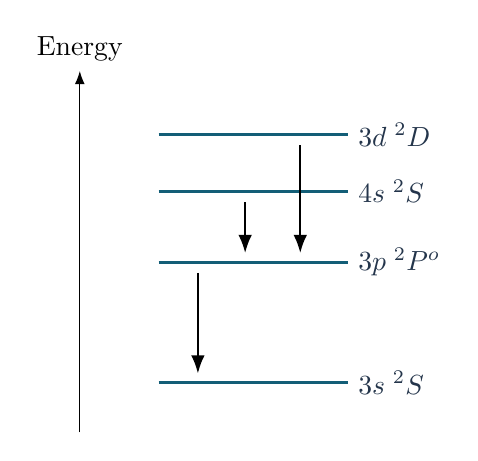
\begin{tikzpicture}[x=1cm,y=.9cm,>=Latex]
\draw[->] (0,0)--(0,5.1) node[above]{Energy};
\draw[accent,very thick](1,0.7)--(3.4,0.7)
node[right,ink]{\(3s\;{}^2S\)};
\draw[accent,very thick](1,2.4)--(3.4,2.4)
node[right,ink]{\(3p\;{}^2P^o\)};
\draw[accent,very thick](1,3.4)--(3.4,3.4)
node[right,ink]{\(4s\;{}^2S\)};
\draw[accent,very thick](1,4.2)--(3.4,4.2)
node[right,ink]{\(3d\;{}^2D\)};
\draw[->,thick] (1.5,2.25)--(1.5,.83);
\draw[->,thick] (2.1,3.25)--(2.1,2.53);
\draw[->,thick] (2.8,4.05)--(2.8,2.53);
\end{tikzpicture}
\]

\subsection*{Step 4: evaluate the radial dipole integrals}
With \(u=rR\), the radial matrix element is
\[
D_{if}=\int_0^\infty u_f(r)\,r\,u_i(r)\diff r.
\]
The numerically computed magnitudes and
transition energies are
\[
\begin{array}{c|r|r}
i\to f&|D_{if}|\ (a_0)&
\omega_{if}=E_i-E_f\ (\mathrm{Ha})\\\hline
3p\to3s&4.48268&0.0729149\\
4s\to3p&4.36430&0.0397087\\
3d\to3p&5.97665&0.0545405
\end{array}
\]
Angular integration over \(Y_{lm}\) supplies
the E1 weights. For a nonrelativistic
spinless orbital with its magnetic substates
appropriately averaged, the total downward
rate is
\[
\boxed{A_{if}=\frac{4\alpha_{\rm fs}^3}{3t_{\rm au}}\,
\omega_{if}^3\,\frac{l_>}{2l_i+1}\,
|D_{if}|^2,}
\]
where \(l_>=\max(l_i,l_f)\),
\(t_{\rm au}=2.4188843266\times10^{-17}\) s.
The factors \(l_>/(2l_i+1)\) are
\(1/3\) for \(p\to s\), \(1\) for
\(s\to p\) and \(2/5\) for \(d\to p\).

\subsection*{Step 5: sum rates and calculate lifetimes}
The excited-state lifetime is
\(\tau_i=[\sum_{f<i}A_{if}]^{-1}\).
With the specified model, each upper state has
one primary orbital E1 channel:
\[
\begin{array}{c|r|r}
i&\text{Calculated }A_i\ (\mathrm{s}^{-1})
&\boxed{\tau_i\ (\mathrm{ns})}\\\hline
3p&5.562\times10^7&17.979\\
4s&2.545\times10^7&39.147\\
3d&4.965\times10^7&20.139
\end{array}
\]
These are independently computed predictions,
not values fitted to the reference lifetimes.

\subsection*{Step 6: compare with published atomic data}
Published nonrelativistic/relativistic
atomic-structure calculations for the Na-like
sequence at \(Z=11\) report approximately
\(16.48\) ns for \(3p\), \(38.25\) ns for
\(4s\), and \(19.67\) ns for \(3d\);
the \(J\)-resolved values vary slightly.
Our percentage differences from these
\emph{theoretical reference} results are:
\[
\begin{array}{c|r|r|r}
&\text{this model (ns)}&
\text{ref. theory (ns)}&
\text{difference}\\\hline
3p&17.979&16.48&+9.10\%\\
4s&39.147&38.25&+2.34\%\\
3d&20.139&19.67&+2.39\%
\end{array}
\]
A separately published direct measurement
of Na I \(3p\) reports \(17.3\pm1.0\) ns,
consistent with our predicted \(17.98\) ns
at that uncertainty. The \(4s\) and \(3d\)
benchmark values in the table are
\emph{calculations}, not claimed direct
measurements; a precise experimental
comparison should use a cited measured
dataset for each fine-structure component.

\subsection*{Step 7: limitations}
This simple model ignores core polarisation,
electron correlation beyond the fitted
potential, spin--orbit fine structure and
configuration mixing. Its chosen \(b\)
parameter controls the radial overlaps;
different fitted potentials change \(\tau\).
Higher multipoles, collisional quenching,
cascades and branching into more levels
may matter outside the minimal model.
Numerical convergence should be checked by
decreasing \(h\) and increasing \(r_{\max}\).

\methodnote{Reproduce every number using
\texttt{python scripts/assignment\_numerical\_solutions.py}.
References: Froese Fischer \emph{et al.},
Atomic Data and Nuclear Data Tables \textbf{92}
(2006), Na-like \(Z=11\) lifetimes;
NIST Na I energy-level table; 1970 JOSA
Na I \(3p\) lifetime measurement.}


\clearpage
\phantomsection
\addcontentsline{toc}{part}{Question-type method finder}
\begin{center}
{\color{accent}\LARGE\bfseries Question-type method finder}
\end{center}
\begin{tabularx}{\linewidth}{@{}p{18mm}X@{}}
\toprule
\textbf{Question}&\textbf{First step to remember}\\\midrule
A1 Q1&Expand \(\ket\Psi\bra\Psi\), trace idler with
\(\delta_{mn}\), differentiate geometric series\\
A1 Q2&Write Fock state using creation operators,
invert the optical mode matrix, apply binomial theorem\\
A2 Q1&Check Bell overlaps, trace one subsystem, transform
both photons to diagonal basis\\
A2 Q2&Apply local Pauli gates, transform \emph{both}
photonic creation operators and classify detector signatures\\
A2 Q3&Sift based on random basis match, condition
intercept--resend error on Alice/Bob matching bases\\
A3 Q1&Form \(\Delta V=V_{\rm finite}-V_{\rm point}\),
integrate over nuclear radius and compare Dirac corrections\\
A3 Q2&Enforce orbital/spin exchange antisymmetry,
count 45 states; check NIST level order\\
A3 Q3&Use second-order Stark expression, symmetry and
closure; convert \(a_0^3\) to polarizability volume\\
A3 Q4&Project \(L,S\to J\), then \(I,J\to F\);
split in \(m_F\) in a weak magnetic field\\
A4 Q1&Separate radial/angular/spin; sum \(m_b,\mu_b\)
before writing Johnson's 3.64 and 3.66\\
A4 Q2&Max scattering force sets \(a_{\max}\);
use \(v\diff v/\diff z\) to test a field profile\\
A4 Q3&Solve the radial tridiagonal Hamiltonian;
calculate E1 angular factors and radial dipoles;
sum rates then invert to lifetime\\\bottomrule
\end{tabularx}

\clearpage
\phantomsection
\addcontentsline{toc}{part}{Reproducible numerical code}
\section*{Appendix: reproducible numerical code}
The following source file is also committed separately
for execution and modification. It calculates the
finite-nuclear-size corrections, Dirac comparison,
and sodium radial energies and lifetimes.
\lstset{language=Python,basicstyle=\ttfamily\scriptsize,
breaklines=true,breakatwhitespace=true,
frame=single,columns=fullflexible,
showstringspaces=false,tabsize=4,
keywordstyle=\color{accent},
commentstyle=\color{gray}}
\lstinputlisting{../../scripts/assignment_numerical_solutions.py}
\end{document}
